\chapter{Sample theory} \label{ch6}
In this chapter sample theory and its importance when converting an analogue audio signal to a digital audio signal along with its complications is treated.
%\section{The frequency domain}
%The following sections look at functions in both the \textit{time}- and \textit{frequency} domains and utilizes the advantages of these different visualizations. To express a function of time as a function of frequency the \textit{Fourier transform} is used. The transform decomposes a periodic function $A$ of time $t$ into an amplitude valued function $\hat{A}$ of frequency $\omega$ and shows which amplitudes of frequencies of different sinusoids are present in the signal. The mathematical background for the Fourier transform is reserved for chapter \ref{ch5} - this chapter will make do with the graphical explanation in figures \ref{fig:time} and \ref{fig:freq}. Notice the both real and imaginary amplitudes of $\hat{A}$.
%\begin{figure}[H]
%\centering
%\begin{minipage}{0.49\textwidth}
%\centering
%\begin{tikzpicture}[scale=0.8]
%\begin{axis}[
%axis lines=middle,
%xtick={-3.14159,3.14159},
%xticklabels={$-\pi$,$\pi$},
%ytick={-1.5,1.5}
%,xmin=-4.25
%,xmax=4.25
%,ymin=-1.75
%,ymax=1.75,
%samples=50]
%\addplot[red][domain=-3.14159:3.14159] {sin(deg(x))+(1/2)*cos(deg(2*x))};
%\end{axis}
%\end{tikzpicture}
%\caption{Graph of $f(x)=\sin x + \frac{1}{2} \cos 2x$ in the time domain.}
%\label{fig:time}
%\end{minipage}
%\centering
%\begin{minipage}{0.49\textwidth}
%\centering
%\begin{tikzpicture}[scale=0.8]
%\begin{axis}[
%axis lines=middle,
%xtick={-6.28318,-3.14159,3.14159,6.28318},
%xticklabels={$-2\pi$,$-\pi$,$\pi$,$2\pi$},
%ytick={-1.5,1.5},
%xmin=-6.75,
%xmax=6.75,
%ymin=-1.75,
%ymax=1.75,]
%\draw[->][red](axis cs:6.28318,0)--(axis cs:6.28318,0.62665);
%\draw[->][red](axis cs:-6.28318,0)--(axis cs:-6.28318,0.62665);
%\draw[->][blue](axis cs:3.14159,0)--(axis cs:3.14159,1.2533);
%\draw[->][blue](axis cs:-3.14159,0)--(axis cs:-3.14159,1.2533);
%\end{axis}
%\end{tikzpicture}
%\caption{Graph of $\hat{f}$ in the frequency domain. Red = real, blue = imaginary.}
%\label{fig:freq}
%\end{minipage}
%\end{figure}
%The above figures illustrate the continuous Fourier transform. The transform can be discretized to the discrete Fourier transform, which is crucial, when working with sampled signals. This is likewise covered in chapter \ref{ch5}.
\section{Sampling}
Sampling is the process of representing a \textit{continuous-time} signal by a sequence of values. Doing so converts the continuous-time signal into a \textit{discrete-time} signal. \cite{pelgrom} The relation between a continuous function $x_c(t)$ and the discrete funtion $x[n]$ obtained by sampling $x_c(t)$ is described by
\begin{equation}\label{eq:sampling_principle}
x[n]=x_c(nT_s)
\end{equation}
where the \textit{sampling period }$T_s$ (time bewteen two consecutive samples) is determined by the \textit{sampling frequency} $f_s$ (samples pr. second). The relation between $T_s$, $f_s$ and the times of samplings is described by
\begin{equation}\label{eq:sample_freq}
t=\frac{n}{f_s}=nT_s, \phantom{mm} n=-\infty,\hdots-1,0,1\hdots,\infty \phantom{mm}\text{\cite{pelgrom}}
\end{equation}
where $n$ is the number of samples.\\\\
To describe sampling mathematically the \textit{Dirac delta} function is introduced in definition \ref{def:dirac}.
\begin{definition}[Dirac delta function]\label{def:dirac}
The Dirac delta function is the function $\delta$ satisfying
\begin{equation}
\int_{-\infty}^{\infty} \! f(t)\delta(t-t_0) \, dt=f(t_0).\phantom{mm}\text{\cite{pelgrom}}
\end{equation}
\end{definition}
Summing an infinite number of Dirac functions shifted at equally spaced time intervals $nT_s$ as in \eqref{eq:dirac_sum} produces a constant function of equidistant Dirac pulses:
\begin{equation}\label{eq:dirac_sum}
s(t)=\sum_{n=-\infty}^{\infty}\delta(t-nT_s)\phantom{mm}\text{\cite{DTSP}}
\end{equation}
Multiplying a continuous signal with \eqref{eq:dirac_sum} and using the property of the Dirac function \eqref{eq:sampling} is obtained:
\begin{align}
x_s(t)&=x_c(t)s(t)\nonumber \\
&=x_c(t)\sum_{n=-\infty}^{\infty}\delta(t - nT_s)\nonumber \\
&=\sum_{n=-\infty}^{\infty}x_c(t)\delta(t - nT_s)\nonumber\\
&=\sum_{n=-\infty}^{\infty}x_c(nT_s)\delta(t - nT_s)\phantom{mm}
\label{eq:sampling}
\end{align}
\eqref{eq:sampling} is a mathematical representation of sampling of the continuous function $x_c(t)$ into the function $x_s(t)$ \cite{DTSP}. Although \eqref{eq:sampling} describes sampling, we have $x_s(t)\neq x[n]$ as $x_s(t)$ is defined in the interval between two samples whereas $x[n]$ only takes values at integers $n$. Although $x_s(t)\neq x[n]$ \eqref{eq:sampling} will be useful in the upcoming appliance of the Fourier transform.
\paragraph{Example of sampling} Sampling a ball following the arc shown in figure \ref{fig:ball_cont} results in the plotted points in figure \ref{fig:ball_disc}. As such the balls path is illustrated with discrete points along the path.
\begin{figure}[H]
\centering
\begin{minipage}{0.49\textwidth}
\centering
\begin{tikzpicture}[scale=1.4]
\draw[->] (-0.25,0) -- (4.25,0) node[right] {$x$};
\draw[->] (0,-0.25) -- (0,2) node[above] {$y$};
\draw[scale=1,domain=0:4,smooth,variable=\x,red] plot ({\x},{-0.25*\x*\x+\x});
\end{tikzpicture}
\caption{Trajectory of a ball described by the time continuous function $x_c(t)$. In continuous time the trajectory is smooth.}
\label{fig:ball_cont}
\end{minipage}
\centering
\begin{minipage}{0.49\textwidth}
\centering
\begin{tikzpicture}[scale=1.4]
\draw[->] (-0.25,0) -- (4.25,0) node[right] {$x$};
\draw[->] (0,-0.25) -- (0,2) node[above] {$y$};
\draw(0,0) node {\textbullet};
\draw(0.5,0.4375) node {\textbullet};
\draw(1,0.75) node {\textbullet};
\draw(1.5,0.9375) node {\textbullet};
\draw(2,1) node {\textbullet};
\draw(2.5,0.9375) node {\textbullet};
\draw(3,0.75) node {\textbullet};
\draw(3.5,0.4375) node {\textbullet};
\draw(4,0) node {\textbullet};
\end{tikzpicture}
\caption{Trajectory of a ball described by the time discrete function $x[n]$. The trajectory consists of samples of $x_c(t)$.}
\label{fig:ball_disc}
\end{minipage}
\end{figure}
\subsection{Frequency representation of sampling}
To study the behavior of $x_s(t)$ in the frequency domain the Fourier transform is used. The Fourier transform of $s(t)$ is seen in \eqref{eq:fourier_impulse}.
\begin{equation}\label{eq:fourier_impulse}
\hat{s}(f)=\frac{2\pi}{T}\sum_{k=-\infty}^{\infty}(f-kf_s)
\end{equation}
The Fourier transform of \eqref{eq:sampling} uses the fact, that \eqref{eq:sampling} is a product of two functions, which is a convolution in the frequency domain:
\begin{equation}
\hat{x}_s(f)=\frac{1}{2\pi}\sum_{k=-\infty}^{\infty}\hat{x}_c(t)(f)*\hat{s}(f)\phantom{mm}\text{\cite{DTSP}}
\end{equation}
It follows \frede{Hvorfor? \texttrademark} that
\begin{equation}\label{eq:samp_freq}
\hat{x}_s(f)=\frac{1}{T}\sum_{k=-\infty}^{\infty}\hat{x}_c(j(f-kf_s))
\end{equation}
\subsection{Aliasing}\label{sec:aliasing}
From \eqref{eq:samp_freq} it is seen that $\hat{x}_s(f)$ consists of copies of $\hat{x}_c$ repeated at whole multiples of $f_s$ on both sides of the origin. From this follows that two different sampled continuous signals may have the same frequency representation. More specifically if the frequencies of two different signals differ from som whole multiple of $f_s$ by the same amount the sequence of samples for the two signals will be identical. \cite{pelgrom} This phenomenon is called aliasing and is illustrated in figures \ref{fig:aliasing1} and \ref{fig:aliasing2} where two sine waves of different frequencies are sampled with the same $f_s$.
\begin{figure}[H]
\centering
\begin{minipage}{0.49\textwidth}
\centering
\begin{tikzpicture}[scale=0.8]
\begin{axis}[
axis lines=middle,
xtick={3.14159,6.28138},
xticklabels={$\pi$,$2\pi$},
ytick={-1,1}
,xmin=-.25
,xmax=6.5
,ymin=-1.25
,ymax=1.25
,samples=50]
\addplot[red][domain=0:6.28318]{sin(deg(x))};
\node at (axis cs:0,0) {\textbullet};
\node at (axis cs:0.6918,0.6428) {\textbullet};
\node at (axis cs:1.3963,0.9848) {\textbullet};
\node at (axis cs:2.0944,0.8660) {\textbullet};
\node at (axis cs:2.7925,0.3420) {\textbullet};
\node at (axis cs:3.4907,-0.3420) {\textbullet};
\node at (axis cs:4.1888,-0.8660) {\textbullet};
\node at (axis cs:4.8869,-0.9848) {\textbullet};
\node at (axis cs:5.5850,-0.6428) {\textbullet};
\node at (axis cs:6.2832,0) {\textbullet};
\end{axis}
\end{tikzpicture}
\caption{Sine wave of angular frequency $\omega=\frac{2\pi}{\text{s}}=1$ Hz sampled at $f_s=9$ Hz.}
\label{fig:aliasing1}
\end{minipage}
\begin{minipage}{0.49\textwidth}
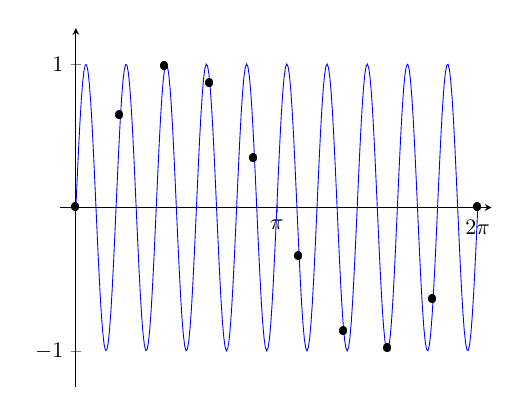
\begin{tikzpicture}[scale=0.8]
\begin{axis}[
axis lines=middle,
xtick={3.14159,6.28138},
xticklabels={$\pi$,$2\pi$},
ytick={-1,1}
,xmin=-.25
,xmax=6.5
,ymin=-1.25
,ymax=1.25
,samples=300]
\addplot[blue][domain=0:6.28138]{sin(deg(10*x))};
\node at (axis cs:0,0) {\textbullet};
\node at (axis cs:0.6918,0.6428) {\textbullet};
\node at (axis cs:1.3963,0.9848) {\textbullet};
\node at (axis cs:2.0944,0.8660) {\textbullet};
\node at (axis cs:2.7925,0.3420) {\textbullet};
\node at (axis cs:3.4907,-0.3420) {\textbullet};
\node at (axis cs:4.1888,-0.8660) {\textbullet};
\node at (axis cs:4.8869,-0.9848) {\textbullet};
\node at (axis cs:5.5850,-0.6428) {\textbullet};
\node at (axis cs:6.2832,0) {\textbullet};
\end{axis}
\end{tikzpicture}
\caption{Sine wave of angular frequency $\omega=\frac{20\pi}{\text{s}}=10$ Hz sampled at $f_s=9$ Hz.}
\label{fig:aliasing2}
\end{minipage}
\end{figure} 
\noindent Aliasing is as noted also shown in the frequency domain - this is seen in figures *Insert references \texttrademark.
\begin{center}
*Insert figures with frequency representation of aliasing \texttrademark*
\end{center}
It is clear, that if $f_s-f_N\geq f_N\Rightarrow f_s\geq2f_N$ there is no overlap of the copies of $\hat{x}_c$. If however $f_s-f_N\leq f_N\Rightarrow f_s\leq 2f_N$ the copies will overlap. The consequence of aliasing is therefore that $x_c$ is not reconstructable from $x_s$ as the above figures and frequency interpretation show.




\section{Analogue-to-digital conversion}\label{ADC}
An analogue-to-digital converter (ADC) is a device which as the name suggests is capable of converting an analogue signal to a digital signal. The analogue signal is in the case of this project voltage from a microphone reacting to sound waves. An audio ADC consists of the following elements
\begin{enumerate}
\item A \textit{track-} or \textit{sample-and-hold} circuit capable of sampling a voltage and \textit{holding} the value during the whole or some part of the sample period.
\end{enumerate}
\begin{figure}[H]
\centering
\begin{tikzpicture}[node distance=3.5cm,auto,>=latex']
\draw
% Drawing the blocks of first filter :
	node at (0,0)[right=-13mm]{\huge\twonotes} % kan skiftet ud med sinus længere nede
	node [input, name=input1] {} 
	node at (input1) [above=5mm] {Mic}		
	node [block, right of=input1] (sh) {$Sampel and hold$}
	node [block, right of=sh] (quant) {$Quantification$}
	node [block, right of=quant] (save) {$Storage$}
	node [sum, right of=save] (cirk1) {}
	node at (cirk1) [above=5mm] {App}
    node [output, name=output1, right of=cirk1]{}
    
    
;
% Joining blocks. 
% Commands \draw with options like [->] must be written individually

\draw[->](input1) -- node {}(sh);
\draw[->](sh) -- node {}(quant);
\draw[->](quant) -- node {}(save);
\draw[->](save) -- node {}(cirk1);
\filldraw[color=black,fill=white,thick](input1) circle (0.3);
\draw(-0.3,0.5) -- (-0.3,-0.5);
%\draw (-1.5,0) sin (-1.40,0.5) cos (-1.30,0) sin (-1.20,-0.5) cos (-1.10,0) sin (-1,0.5) cos (-0.9,0) sin (-0.8,-0.5) cos (-0.7,0);

% Boxing and labelling noise shapers
\draw [color=gray,thick,dashed](1.5,-1.5) rectangle (9,1.5);
\node at (1.5,1.7) [above=5mm, right=0mm] {\textsc{ADC}};
\end{tikzpicture}
\caption{Basic block-diagram illustrating an ADC where the digital output will be the input to the application} 
\label{fig:input}
\end{figure}
%\input{sections/mainmatter/chapter_4/_____.tex}




\clearpage
\section{Noise}
About noise from chapter 2: \textregistered

Playing a pitch alone in an anechoic room is a way of minimizing noise factors. There are many different noise sources from e.g. the surrounding environment, electrical equipment, other people and even the instrument playing itself since it is difficult to make a pure tone by an acoustic sound source such as a guitar. A pure tone is a sinusoidal waveform consisting of a single frequency and may therefore be difficult to play on an instrument. \cite{AcousticNoise} Usually, sound is reflected off the walls in a room which is also a source of noise. This is a form of folding and is minimized in the anechoic room because sound is absorbed by the walls. Moreover, due to the construction of the anechoic room, noise from e.g. bypassing cars is also minimized, and the sound may be recorded with a minimum of hardware which otherwise may also produce noise.
\\ \\
The music used in this project will therefore be recorded in an anechoic room because the noise is minimized. It is not expected that musicians using the system in the future have access to an anechoic room as well but if the system doesn't work with sounds recorded in the anechoic room then it with most certainty doesn't work at other places neither. However, in order to reproduce the conditions of a typical musician working around other people, background noise can also be made in the anechoic room but should of course not drown the music. This form of noise is additive whereas e.g. noise reflected off walls as mentioned above is multiplicative. In general, multiplicative noise depends on the state of the system whereas additive noise does not. Therefore, the output $x[n]$ of the sampled data $s[n]$ corrupted by the additive noise $a[n]$ is $x[n] = s[n] + a[n]$ whereas the equation for the multiplicative noise $m[n]$ is $x[n] = s[n]m[n]$.